% Options for packages loaded elsewhere
\PassOptionsToPackage{unicode}{hyperref}
\PassOptionsToPackage{hyphens}{url}
%
\documentclass[
]{article}
\usepackage{amsmath,amssymb}
\usepackage{iftex}
\ifPDFTeX
  \usepackage[T1]{fontenc}
  \usepackage[utf8]{inputenc}
  \usepackage{textcomp} % provide euro and other symbols
\else % if luatex or xetex
  \usepackage{unicode-math} % this also loads fontspec
  \defaultfontfeatures{Scale=MatchLowercase}
  \defaultfontfeatures[\rmfamily]{Ligatures=TeX,Scale=1}
\fi
\usepackage{lmodern}
\ifPDFTeX\else
  % xetex/luatex font selection
\fi
% Use upquote if available, for straight quotes in verbatim environments
\IfFileExists{upquote.sty}{\usepackage{upquote}}{}
\IfFileExists{microtype.sty}{% use microtype if available
  \usepackage[]{microtype}
  \UseMicrotypeSet[protrusion]{basicmath} % disable protrusion for tt fonts
}{}
\makeatletter
\@ifundefined{KOMAClassName}{% if non-KOMA class
  \IfFileExists{parskip.sty}{%
    \usepackage{parskip}
  }{% else
    \setlength{\parindent}{0pt}
    \setlength{\parskip}{6pt plus 2pt minus 1pt}}
}{% if KOMA class
  \KOMAoptions{parskip=half}}
\makeatother
\usepackage{xcolor}
\usepackage[margin=1in]{geometry}
\usepackage{color}
\usepackage{fancyvrb}
\newcommand{\VerbBar}{|}
\newcommand{\VERB}{\Verb[commandchars=\\\{\}]}
\DefineVerbatimEnvironment{Highlighting}{Verbatim}{commandchars=\\\{\}}
% Add ',fontsize=\small' for more characters per line
\usepackage{framed}
\definecolor{shadecolor}{RGB}{248,248,248}
\newenvironment{Shaded}{\begin{snugshade}}{\end{snugshade}}
\newcommand{\AlertTok}[1]{\textcolor[rgb]{0.94,0.16,0.16}{#1}}
\newcommand{\AnnotationTok}[1]{\textcolor[rgb]{0.56,0.35,0.01}{\textbf{\textit{#1}}}}
\newcommand{\AttributeTok}[1]{\textcolor[rgb]{0.13,0.29,0.53}{#1}}
\newcommand{\BaseNTok}[1]{\textcolor[rgb]{0.00,0.00,0.81}{#1}}
\newcommand{\BuiltInTok}[1]{#1}
\newcommand{\CharTok}[1]{\textcolor[rgb]{0.31,0.60,0.02}{#1}}
\newcommand{\CommentTok}[1]{\textcolor[rgb]{0.56,0.35,0.01}{\textit{#1}}}
\newcommand{\CommentVarTok}[1]{\textcolor[rgb]{0.56,0.35,0.01}{\textbf{\textit{#1}}}}
\newcommand{\ConstantTok}[1]{\textcolor[rgb]{0.56,0.35,0.01}{#1}}
\newcommand{\ControlFlowTok}[1]{\textcolor[rgb]{0.13,0.29,0.53}{\textbf{#1}}}
\newcommand{\DataTypeTok}[1]{\textcolor[rgb]{0.13,0.29,0.53}{#1}}
\newcommand{\DecValTok}[1]{\textcolor[rgb]{0.00,0.00,0.81}{#1}}
\newcommand{\DocumentationTok}[1]{\textcolor[rgb]{0.56,0.35,0.01}{\textbf{\textit{#1}}}}
\newcommand{\ErrorTok}[1]{\textcolor[rgb]{0.64,0.00,0.00}{\textbf{#1}}}
\newcommand{\ExtensionTok}[1]{#1}
\newcommand{\FloatTok}[1]{\textcolor[rgb]{0.00,0.00,0.81}{#1}}
\newcommand{\FunctionTok}[1]{\textcolor[rgb]{0.13,0.29,0.53}{\textbf{#1}}}
\newcommand{\ImportTok}[1]{#1}
\newcommand{\InformationTok}[1]{\textcolor[rgb]{0.56,0.35,0.01}{\textbf{\textit{#1}}}}
\newcommand{\KeywordTok}[1]{\textcolor[rgb]{0.13,0.29,0.53}{\textbf{#1}}}
\newcommand{\NormalTok}[1]{#1}
\newcommand{\OperatorTok}[1]{\textcolor[rgb]{0.81,0.36,0.00}{\textbf{#1}}}
\newcommand{\OtherTok}[1]{\textcolor[rgb]{0.56,0.35,0.01}{#1}}
\newcommand{\PreprocessorTok}[1]{\textcolor[rgb]{0.56,0.35,0.01}{\textit{#1}}}
\newcommand{\RegionMarkerTok}[1]{#1}
\newcommand{\SpecialCharTok}[1]{\textcolor[rgb]{0.81,0.36,0.00}{\textbf{#1}}}
\newcommand{\SpecialStringTok}[1]{\textcolor[rgb]{0.31,0.60,0.02}{#1}}
\newcommand{\StringTok}[1]{\textcolor[rgb]{0.31,0.60,0.02}{#1}}
\newcommand{\VariableTok}[1]{\textcolor[rgb]{0.00,0.00,0.00}{#1}}
\newcommand{\VerbatimStringTok}[1]{\textcolor[rgb]{0.31,0.60,0.02}{#1}}
\newcommand{\WarningTok}[1]{\textcolor[rgb]{0.56,0.35,0.01}{\textbf{\textit{#1}}}}
\usepackage{graphicx}
\makeatletter
\def\maxwidth{\ifdim\Gin@nat@width>\linewidth\linewidth\else\Gin@nat@width\fi}
\def\maxheight{\ifdim\Gin@nat@height>\textheight\textheight\else\Gin@nat@height\fi}
\makeatother
% Scale images if necessary, so that they will not overflow the page
% margins by default, and it is still possible to overwrite the defaults
% using explicit options in \includegraphics[width, height, ...]{}
\setkeys{Gin}{width=\maxwidth,height=\maxheight,keepaspectratio}
% Set default figure placement to htbp
\makeatletter
\def\fps@figure{htbp}
\makeatother
\setlength{\emergencystretch}{3em} % prevent overfull lines
\providecommand{\tightlist}{%
  \setlength{\itemsep}{0pt}\setlength{\parskip}{0pt}}
\setcounter{secnumdepth}{-\maxdimen} % remove section numbering
\ifLuaTeX
  \usepackage{selnolig}  % disable illegal ligatures
\fi
\IfFileExists{bookmark.sty}{\usepackage{bookmark}}{\usepackage{hyperref}}
\IfFileExists{xurl.sty}{\usepackage{xurl}}{} % add URL line breaks if available
\urlstyle{same}
\hypersetup{
  pdftitle={data\_analysis\_for\_McManus},
  pdfauthor={Siqi},
  hidelinks,
  pdfcreator={LaTeX via pandoc}}

\title{data\_analysis\_for\_McManus}
\author{Siqi}
\date{2024-10-21}

\begin{document}
\maketitle

\hypertarget{r-markdown}{%
\subsection{R Markdown}\label{r-markdown}}

\begin{Shaded}
\begin{Highlighting}[]
\CommentTok{\# Load necessary libraries}
\FunctionTok{set.seed}\NormalTok{(}\DecValTok{123}\NormalTok{)}
\FunctionTok{library}\NormalTok{(ggplot2)}
\FunctionTok{library}\NormalTok{(splines)}
\FunctionTok{library}\NormalTok{(minpack.lm)}
\CommentTok{\#install.packages("pracma") }
\FunctionTok{library}\NormalTok{(pracma)}
\end{Highlighting}
\end{Shaded}

\hypertarget{including-plots}{%
\subsection{Including Plots}\label{including-plots}}

Data Cleaning and Plotting

\begin{Shaded}
\begin{Highlighting}[]
\CommentTok{\# Load and process the  }
\FunctionTok{library}\NormalTok{(readxl)}
\NormalTok{Data\_McManus2\_WT\_P2L\_AAVCremCherry }\OtherTok{\textless{}{-}} \FunctionTok{read\_excel}\NormalTok{(}\StringTok{"/Users/angelzhang/Downloads/CircadianProject/Data\_McManus2\_WT\_P2L\_AAVCremCherry.xlsx"}\NormalTok{)}
\end{Highlighting}
\end{Shaded}

\begin{verbatim}
## New names:
## * `` -> `...1`
\end{verbatim}

\begin{Shaded}
\begin{Highlighting}[]
\NormalTok{df\_MC }\OtherTok{\textless{}{-}} \FunctionTok{as.data.frame}\NormalTok{(Data\_McManus2\_WT\_P2L\_AAVCremCherry)}

\CommentTok{\# Rename columns for clarity}
\FunctionTok{colnames}\NormalTok{(df\_MC) }\OtherTok{\textless{}{-}} \FunctionTok{c}\NormalTok{(}\StringTok{"Time"}\NormalTok{, }\StringTok{"X1"}\NormalTok{, }\StringTok{"X2"}\NormalTok{, }\StringTok{"X3"}\NormalTok{, }\StringTok{"X4"}\NormalTok{)}

\CommentTok{\# Remove outliers where Time is between 100 and 100.1}
\NormalTok{df\_MC }\OtherTok{\textless{}{-}}\NormalTok{ df\_MC[}\SpecialCharTok{!}\NormalTok{(df\_MC}\SpecialCharTok{$}\NormalTok{Time }\SpecialCharTok{\textgreater{}=} \DecValTok{100} \SpecialCharTok{\&}\NormalTok{ df\_MC}\SpecialCharTok{$}\NormalTok{Time }\SpecialCharTok{\textless{}=} \FloatTok{100.1}\NormalTok{), ]}

\CommentTok{\# Plot each species}
\FunctionTok{ggplot}\NormalTok{(df\_MC, }\FunctionTok{aes}\NormalTok{(}\AttributeTok{x =}\NormalTok{ Time)) }\SpecialCharTok{+}
  \FunctionTok{geom\_line}\NormalTok{(}\FunctionTok{aes}\NormalTok{(}\AttributeTok{y =}\NormalTok{ X1, }\AttributeTok{color =} \StringTok{"X1"}\NormalTok{)) }\SpecialCharTok{+}
  \FunctionTok{geom\_line}\NormalTok{(}\FunctionTok{aes}\NormalTok{(}\AttributeTok{y =}\NormalTok{ X2, }\AttributeTok{color =} \StringTok{"X2"}\NormalTok{)) }\SpecialCharTok{+}
  \FunctionTok{geom\_line}\NormalTok{(}\FunctionTok{aes}\NormalTok{(}\AttributeTok{y =}\NormalTok{ X3, }\AttributeTok{color =} \StringTok{"X3"}\NormalTok{)) }\SpecialCharTok{+}
  \FunctionTok{geom\_line}\NormalTok{(}\FunctionTok{aes}\NormalTok{(}\AttributeTok{y =}\NormalTok{ X4, }\AttributeTok{color =} \StringTok{"X4"}\NormalTok{)) }\SpecialCharTok{+}
  \FunctionTok{labs}\NormalTok{(}\AttributeTok{title =} \StringTok{"Data without Outliers"}\NormalTok{, }\AttributeTok{x =} \StringTok{"Time"}\NormalTok{, }\AttributeTok{y =} \StringTok{"X(t\_i)"}\NormalTok{) }\SpecialCharTok{+}
  \FunctionTok{scale\_color\_manual}\NormalTok{(}\AttributeTok{values =} \FunctionTok{c}\NormalTok{(}\StringTok{"X1"} \OtherTok{=} \StringTok{"blue"}\NormalTok{, }\StringTok{"X2"} \OtherTok{=} \StringTok{"green"}\NormalTok{, }\StringTok{"X3"} \OtherTok{=} \StringTok{"red"}\NormalTok{, }\StringTok{"X4"} \OtherTok{=} \StringTok{"purple"}\NormalTok{)) }\SpecialCharTok{+}
  \FunctionTok{theme\_minimal}\NormalTok{()}
\end{Highlighting}
\end{Shaded}

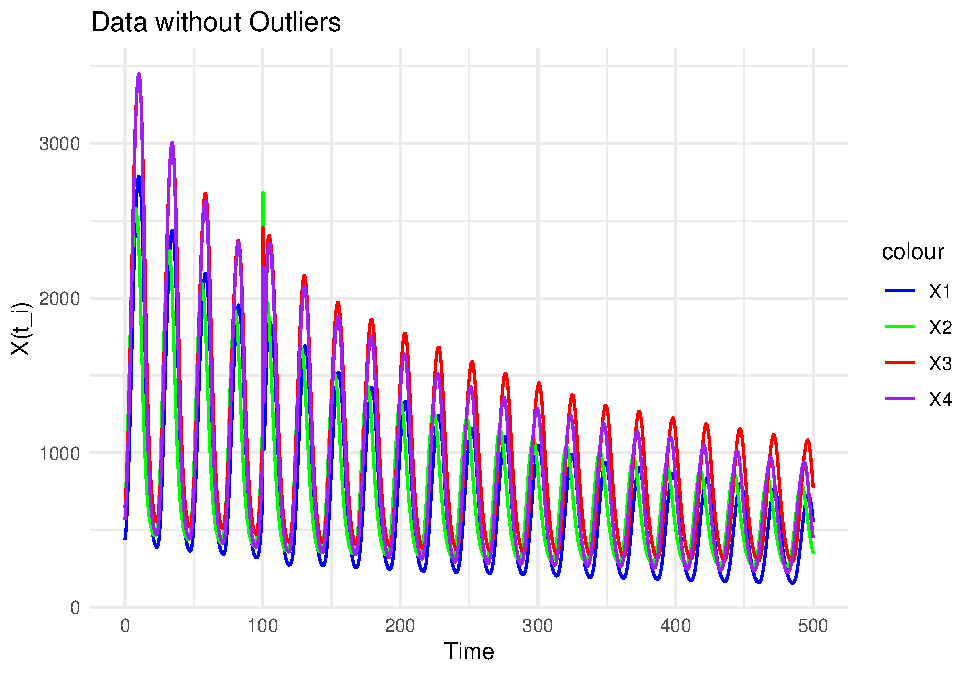
\includegraphics{CircadianProjectForMcManus_files/figure-latex/unnamed-chunk-2-1.pdf}

\begin{Shaded}
\begin{Highlighting}[]
\NormalTok{spline\_X1 }\OtherTok{\textless{}{-}} \FunctionTok{predict}\NormalTok{(}\FunctionTok{smooth.spline}\NormalTok{(df\_MC}\SpecialCharTok{$}\NormalTok{Time, df\_MC}\SpecialCharTok{$}\NormalTok{X1),    }\AttributeTok{spar =}\NormalTok{)}
\NormalTok{spline\_X2 }\OtherTok{\textless{}{-}} \FunctionTok{predict}\NormalTok{(}\FunctionTok{smooth.spline}\NormalTok{(df\_MC}\SpecialCharTok{$}\NormalTok{Time, df\_MC}\SpecialCharTok{$}\NormalTok{X2))}
\NormalTok{spline\_X3 }\OtherTok{\textless{}{-}} \FunctionTok{predict}\NormalTok{(}\FunctionTok{smooth.spline}\NormalTok{(df\_MC}\SpecialCharTok{$}\NormalTok{Time, df\_MC}\SpecialCharTok{$}\NormalTok{X3))}
\NormalTok{spline\_X4 }\OtherTok{\textless{}{-}} \FunctionTok{predict}\NormalTok{(}\FunctionTok{smooth.spline}\NormalTok{(df\_MC}\SpecialCharTok{$}\NormalTok{Time,df\_MC}\SpecialCharTok{$}\NormalTok{X4))}

\CommentTok{\# Plot the spline{-}smoothed data}
\FunctionTok{plot}\NormalTok{(df\_MC}\SpecialCharTok{$}\NormalTok{Time, spline\_X1}\SpecialCharTok{$}\NormalTok{y, }\AttributeTok{type =} \StringTok{"l"}\NormalTok{, }\AttributeTok{col =} \StringTok{"red"}\NormalTok{, }\AttributeTok{lwd =} \DecValTok{2}\NormalTok{, }
     \AttributeTok{xlab =} \StringTok{"Time"}\NormalTok{, }\AttributeTok{ylab =} \StringTok{"Values"}\NormalTok{, }\AttributeTok{main =} \StringTok{" Splines"}\NormalTok{, }
     \AttributeTok{ylim =} \FunctionTok{range}\NormalTok{(}\FunctionTok{c}\NormalTok{(spline\_X1}\SpecialCharTok{$}\NormalTok{y, spline\_X2}\SpecialCharTok{$}\NormalTok{y, spline\_X3}\SpecialCharTok{$}\NormalTok{y, spline\_X4)))}
\FunctionTok{lines}\NormalTok{(df\_MC}\SpecialCharTok{$}\NormalTok{Time, spline\_X2}\SpecialCharTok{$}\NormalTok{y, }\AttributeTok{col =} \StringTok{"blue"}\NormalTok{, }\AttributeTok{lwd =} \DecValTok{2}\NormalTok{)}
\FunctionTok{lines}\NormalTok{(df\_MC}\SpecialCharTok{$}\NormalTok{Time, spline\_X3}\SpecialCharTok{$}\NormalTok{y, }\AttributeTok{col =} \StringTok{"green"}\NormalTok{, }\AttributeTok{lwd =} \DecValTok{2}\NormalTok{)}
\FunctionTok{lines}\NormalTok{(df\_MC}\SpecialCharTok{$}\NormalTok{Time, spline\_X4}\SpecialCharTok{$}\NormalTok{y, }\AttributeTok{col =} \StringTok{"purple"}\NormalTok{, }\AttributeTok{lwd =} \DecValTok{2}\NormalTok{)}

\FunctionTok{legend}\NormalTok{(}\StringTok{"topright"}\NormalTok{, }\AttributeTok{legend =} \FunctionTok{c}\NormalTok{(}\StringTok{"spline\_X1"}\NormalTok{, }\StringTok{"spline\_X2"}\NormalTok{, }\StringTok{"spline\_X3"}\NormalTok{, }\StringTok{"spline\_X4"}\NormalTok{), }
       \AttributeTok{col =} \FunctionTok{c}\NormalTok{(}\StringTok{"red"}\NormalTok{, }\StringTok{"blue"}\NormalTok{, }\StringTok{"green"}\NormalTok{, }\StringTok{"purple"}\NormalTok{), }\AttributeTok{lwd =} \DecValTok{2}\NormalTok{)}
\end{Highlighting}
\end{Shaded}

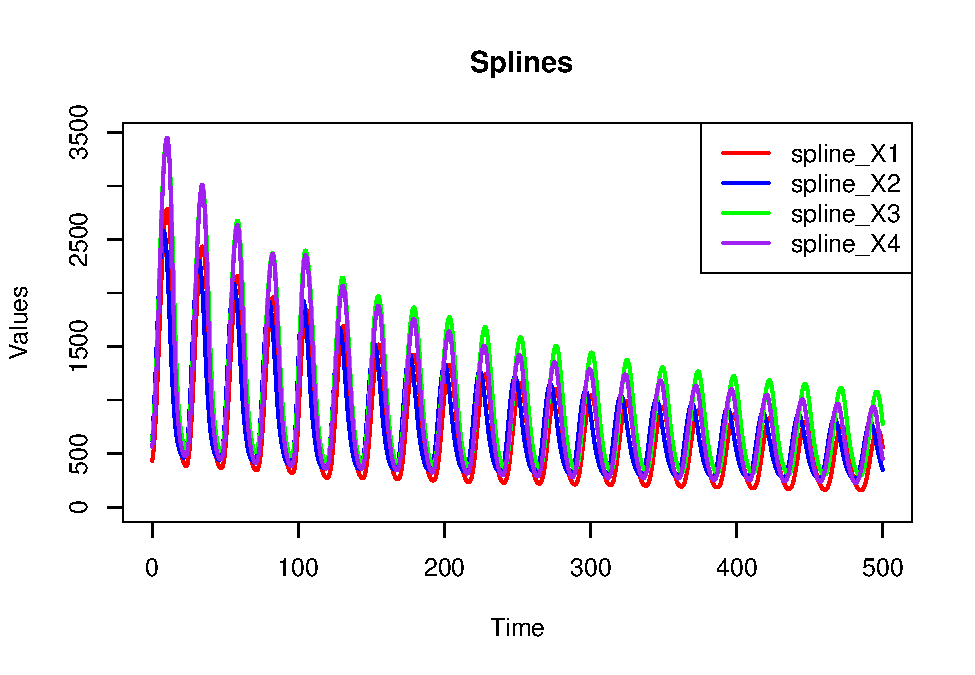
\includegraphics{CircadianProjectForMcManus_files/figure-latex/unnamed-chunk-3-1.pdf}

\begin{Shaded}
\begin{Highlighting}[]
\CommentTok{\# Plot the spline{-}smoothed data}
\NormalTok{spline\_X1 }\OtherTok{\textless{}{-}} \FunctionTok{predict}\NormalTok{(}\FunctionTok{smooth.spline}\NormalTok{(df\_MC}\SpecialCharTok{$}\NormalTok{Time, df\_MC}\SpecialCharTok{$}\NormalTok{X1, }\AttributeTok{spar=}\DecValTok{1}\NormalTok{)) }\CommentTok{\#black line in 2nd \#plot(average for X1)}

\FunctionTok{plot}\NormalTok{(df\_MC}\SpecialCharTok{$}\NormalTok{Time, df\_MC}\SpecialCharTok{$}\NormalTok{X1, }\AttributeTok{type =} \StringTok{"l"}\NormalTok{, }\AttributeTok{col =} \StringTok{"yellow"}\NormalTok{, }\AttributeTok{lwd =} \DecValTok{2}\NormalTok{, }
     \AttributeTok{xlab =} \StringTok{"Time"}\NormalTok{, }\AttributeTok{ylab =} \StringTok{"Values"}\NormalTok{, }\AttributeTok{main =} \StringTok{" Splines"}\NormalTok{, }
     \AttributeTok{ylim =} \FunctionTok{range}\NormalTok{(}\FunctionTok{c}\NormalTok{(spline\_X1}\SpecialCharTok{$}\NormalTok{y, spline\_X2}\SpecialCharTok{$}\NormalTok{y, spline\_X3}\SpecialCharTok{$}\NormalTok{y, spline\_X4)))}
\FunctionTok{lines}\NormalTok{(df\_MC}\SpecialCharTok{$}\NormalTok{Time, spline\_X1}\SpecialCharTok{$}\NormalTok{y)}
\end{Highlighting}
\end{Shaded}

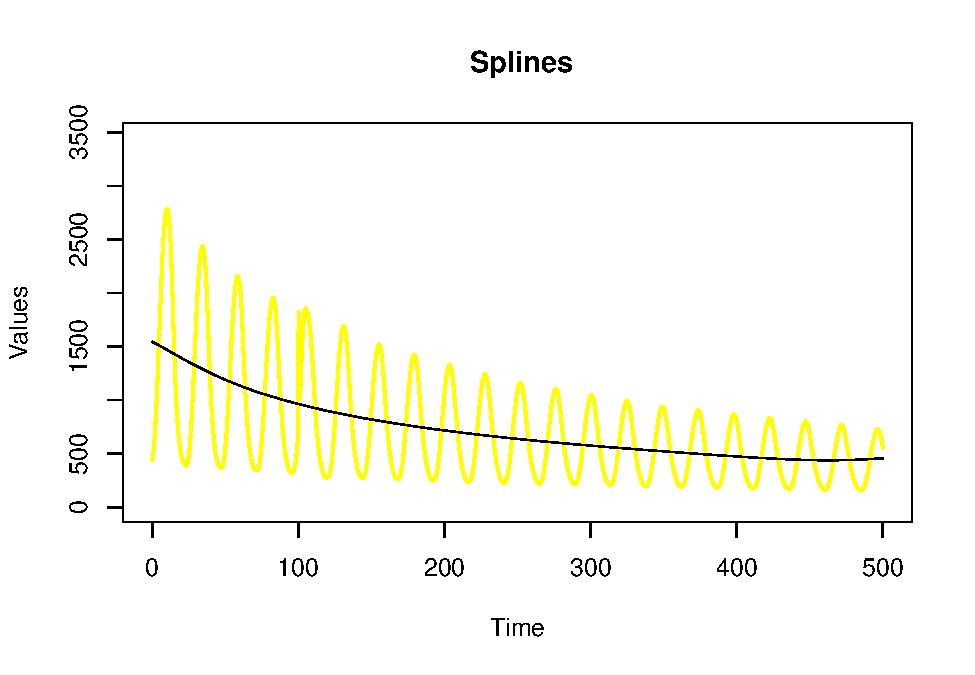
\includegraphics{CircadianProjectForMcManus_files/figure-latex/unnamed-chunk-3-2.pdf}

\begin{Shaded}
\begin{Highlighting}[]
\FunctionTok{plot}\NormalTok{(df\_MC}\SpecialCharTok{$}\NormalTok{Time, df\_MC}\SpecialCharTok{$}\NormalTok{X1}\SpecialCharTok{{-}}\NormalTok{spline\_X1}\SpecialCharTok{$}\NormalTok{y, }\AttributeTok{type =} \StringTok{"l"}\NormalTok{, }\AttributeTok{col =} \StringTok{"yellow"}\NormalTok{, }\AttributeTok{lwd =} \DecValTok{2}\NormalTok{, }
     \AttributeTok{xlab =} \StringTok{"Time"}\NormalTok{, }\AttributeTok{ylab =} \StringTok{"Values"}\NormalTok{, }\AttributeTok{main =} \StringTok{" Detrended Splines"}\NormalTok{)}
\end{Highlighting}
\end{Shaded}

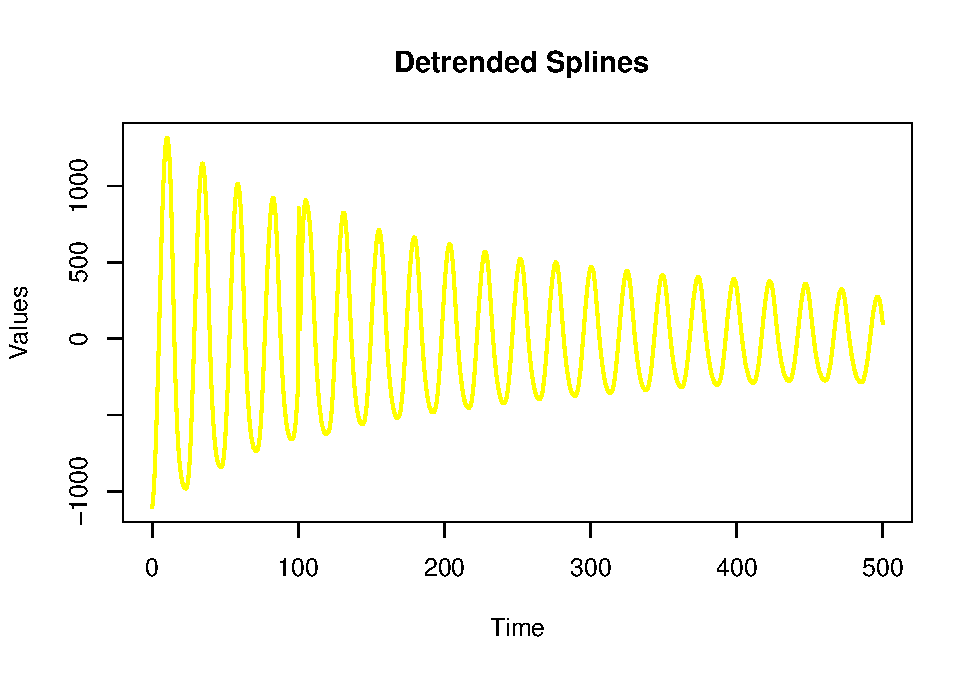
\includegraphics{CircadianProjectForMcManus_files/figure-latex/unnamed-chunk-3-3.pdf}

\begin{Shaded}
\begin{Highlighting}[]
\NormalTok{x }\OtherTok{\textless{}{-}} \DecValTok{1}\SpecialCharTok{:}\FunctionTok{length}\NormalTok{(df\_MC}\SpecialCharTok{$}\NormalTok{Time)  }
\NormalTok{y }\OtherTok{\textless{}{-}}\NormalTok{ df\_MC}\SpecialCharTok{$}\NormalTok{X1}\SpecialCharTok{{-}}\NormalTok{spline\_X1}\SpecialCharTok{$}\NormalTok{y    }

\NormalTok{maxima }\OtherTok{\textless{}{-}} \FunctionTok{findpeaks}\NormalTok{(df\_MC}\SpecialCharTok{$}\NormalTok{X1}\SpecialCharTok{{-}}\NormalTok{spline\_X1}\SpecialCharTok{$}\NormalTok{y, }\AttributeTok{minpeakheight=}\DecValTok{0}\NormalTok{)  }
\NormalTok{minima }\OtherTok{\textless{}{-}} \FunctionTok{findpeaks}\NormalTok{(}\SpecialCharTok{{-}}\NormalTok{df\_MC}\SpecialCharTok{$}\NormalTok{X1}\SpecialCharTok{{-}}\NormalTok{spline\_X1}\SpecialCharTok{$}\NormalTok{y, }\AttributeTok{minpeakheight=}\DecValTok{0}\NormalTok{) }

\NormalTok{x\_max }\OtherTok{\textless{}{-}}\NormalTok{ maxima[,}\DecValTok{2}\NormalTok{]  }
\NormalTok{y\_max }\OtherTok{\textless{}{-}}\NormalTok{ maxima[,}\DecValTok{1}\NormalTok{]  }


\NormalTok{fit }\OtherTok{\textless{}{-}} \FunctionTok{nls}\NormalTok{(y\_max }\SpecialCharTok{\textasciitilde{}}\NormalTok{ a }\SpecialCharTok{*} \FunctionTok{exp}\NormalTok{(}\SpecialCharTok{{-}}\NormalTok{b }\SpecialCharTok{*}\NormalTok{ x\_max) }\SpecialCharTok{+}\NormalTok{ c, }\AttributeTok{start =} \FunctionTok{list}\NormalTok{(}\AttributeTok{a =} \FunctionTok{max}\NormalTok{(y\_max), }\AttributeTok{b =} \FloatTok{0.01}\NormalTok{, }\AttributeTok{c =} \FunctionTok{min}\NormalTok{(y\_max)))}

\FunctionTok{summary}\NormalTok{(fit)}
\end{Highlighting}
\end{Shaded}

\begin{verbatim}
## 
## Formula: y_max ~ a * exp(-b * x_max) + c
## 
## Parameters:
##    Estimate Std. Error t value Pr(>|t|)    
## a 1.115e+03  9.552e+00  116.69   <2e-16 ***
## b 5.000e-04  1.421e-05   35.18   <2e-16 ***
## c 2.142e+02  1.051e+01   20.37   <2e-16 ***
## ---
## Signif. codes:  0 '***' 0.001 '**' 0.01 '*' 0.05 '.' 0.1 ' ' 1
## 
## Residual standard error: 21.65 on 98 degrees of freedom
## 
## Number of iterations to convergence: 13 
## Achieved convergence tolerance: 5.184e-06
\end{verbatim}

\begin{Shaded}
\begin{Highlighting}[]
\NormalTok{a }\OtherTok{\textless{}{-}} \FunctionTok{coef}\NormalTok{(fit)[}\StringTok{"a"}\NormalTok{]}
\NormalTok{b }\OtherTok{\textless{}{-}} \FunctionTok{coef}\NormalTok{(fit)[}\StringTok{"b"}\NormalTok{]}
\NormalTok{c }\OtherTok{\textless{}{-}} \FunctionTok{coef}\NormalTok{(fit)[}\StringTok{"c"}\NormalTok{]}

\FunctionTok{plot}\NormalTok{(x, y, }\AttributeTok{type=}\StringTok{"l"}\NormalTok{, }\AttributeTok{col=}\StringTok{"yellow"}\NormalTok{, }\AttributeTok{main=}\StringTok{"Detrended Splines with Exponential Fit"}\NormalTok{)}
\FunctionTok{lines}\NormalTok{(x\_max, }\FunctionTok{predict}\NormalTok{(fit, }\FunctionTok{list}\NormalTok{(}\AttributeTok{x\_max =}\NormalTok{ x\_max)), }\AttributeTok{col=}\StringTok{"red"}\NormalTok{, }\AttributeTok{lwd=}\DecValTok{2}\NormalTok{)  }\CommentTok{\#}
\end{Highlighting}
\end{Shaded}

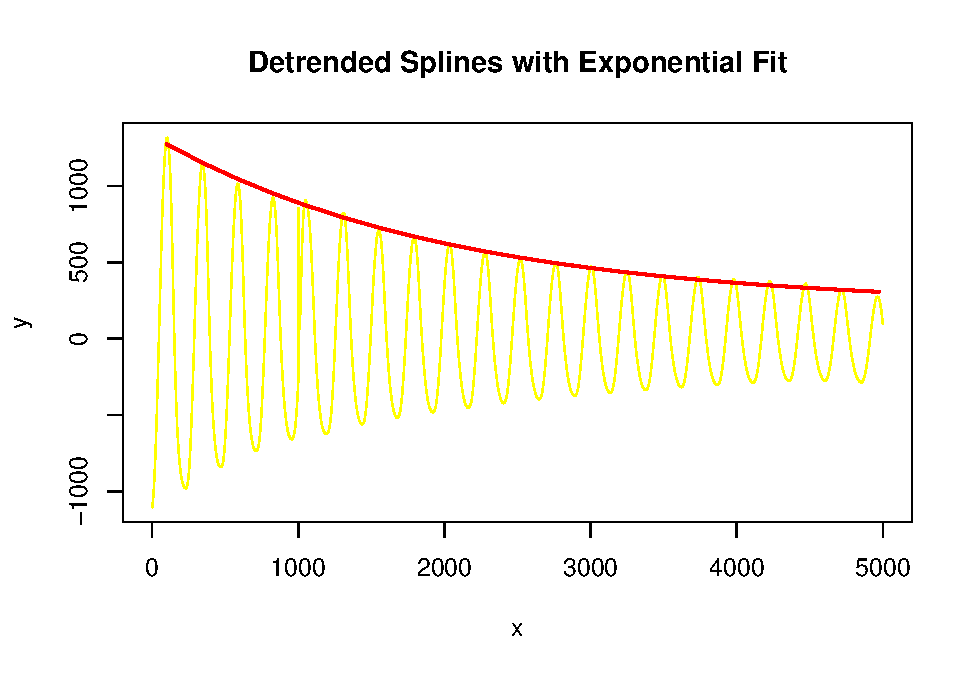
\includegraphics{CircadianProjectForMcManus_files/figure-latex/unnamed-chunk-4-1.pdf}

Simulate Data Based on the Fitted Model

\begin{Shaded}
\begin{Highlighting}[]
\NormalTok{t }\OtherTok{\textless{}{-}} \FunctionTok{seq}\NormalTok{(}\DecValTok{0}\NormalTok{, }\DecValTok{100}\NormalTok{, }\AttributeTok{by =} \FloatTok{0.1}\NormalTok{)}

\NormalTok{model\_function }\OtherTok{\textless{}{-}} \ControlFlowTok{function}\NormalTok{(t, A, gamma, omega, phi, y\_shift) \{}
\NormalTok{  A }\SpecialCharTok{*} \FunctionTok{exp}\NormalTok{(}\SpecialCharTok{{-}}\NormalTok{gamma }\SpecialCharTok{*}\NormalTok{ t ) }\SpecialCharTok{*} \FunctionTok{cos}\NormalTok{(omega }\SpecialCharTok{*}\NormalTok{ t }\SpecialCharTok{+}\NormalTok{ phi) }\SpecialCharTok{+}\NormalTok{ y\_shift}
\NormalTok{\}}

\CommentTok{\# using estimated parameters to def simulating function}
\NormalTok{simulate\_data }\OtherTok{\textless{}{-}} \ControlFlowTok{function}\NormalTok{(t, params, sigma) \{}
\NormalTok{  predicted }\OtherTok{\textless{}{-}} \FunctionTok{model\_function}\NormalTok{(t, params[}\DecValTok{1}\NormalTok{], params[}\DecValTok{2}\NormalTok{], params[}\DecValTok{3}\NormalTok{], params[}\DecValTok{4}\NormalTok{], params[}\DecValTok{5}\NormalTok{])}
\NormalTok{  noise }\OtherTok{\textless{}{-}} \FunctionTok{rnorm}\NormalTok{(}\FunctionTok{length}\NormalTok{(t), }\AttributeTok{mean =} \DecValTok{0}\NormalTok{, }\AttributeTok{sd =}\NormalTok{ sigma)  }\CommentTok{\#using sigma0 to produce noise }
\NormalTok{  simulated\_data }\OtherTok{\textless{}{-}}\NormalTok{ predicted }\SpecialCharTok{+}\NormalTok{ noise}
  \FunctionTok{return}\NormalTok{(simulated\_data)}
\NormalTok{\}}
\NormalTok{sigma0 }\OtherTok{=} \DecValTok{10}
\NormalTok{param0}\OtherTok{=}\FunctionTok{c}\NormalTok{(}\DecValTok{1000}\NormalTok{, }\FloatTok{0.025}\NormalTok{, }\FloatTok{0.9}\NormalTok{, }\DecValTok{0}\NormalTok{,}\DecValTok{0}\NormalTok{)}
\NormalTok{simulated\_data }\OtherTok{\textless{}{-}} \FunctionTok{simulate\_data}\NormalTok{(t, param0, sigma0 )}
\end{Highlighting}
\end{Shaded}

\begin{Shaded}
\begin{Highlighting}[]
\FunctionTok{plot}\NormalTok{(t, simulated\_data, }\AttributeTok{type =} \StringTok{"l"}\NormalTok{, }\AttributeTok{col =} \StringTok{"blue"}\NormalTok{, }\AttributeTok{main =} \StringTok{"Simulated Data"}\NormalTok{, }\AttributeTok{xlab =} \StringTok{"Time"}\NormalTok{, }\AttributeTok{ylab =} \StringTok{"Simulated Values"}\NormalTok{)}
\end{Highlighting}
\end{Shaded}

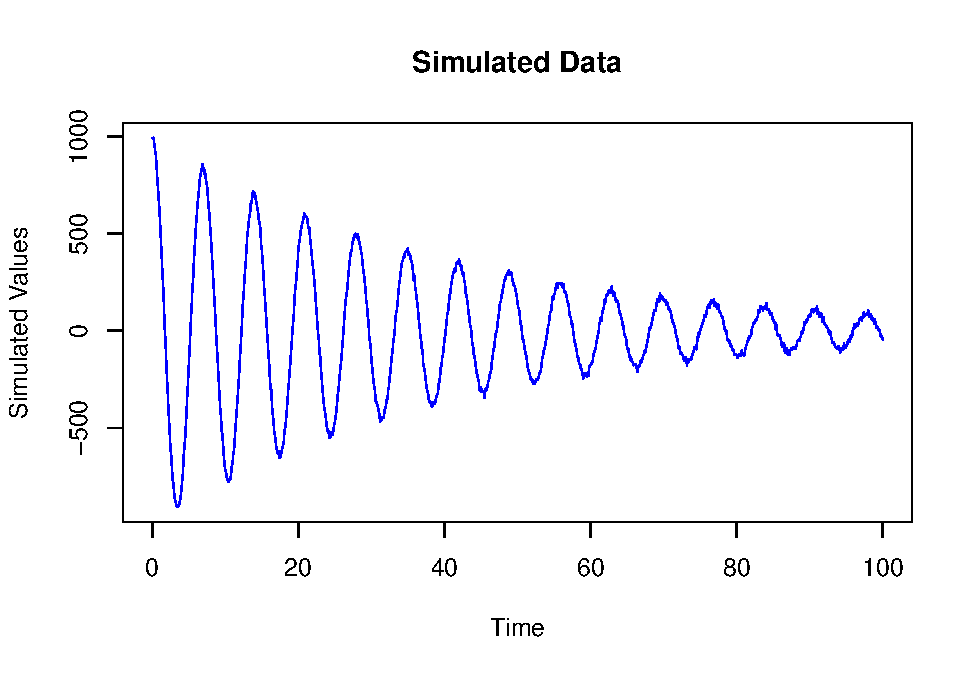
\includegraphics{CircadianProjectForMcManus_files/figure-latex/unnamed-chunk-7-1.pdf}

\#\#Task1 \#\#generate simulating data 1 time

\begin{Shaded}
\begin{Highlighting}[]
\NormalTok{true\_params }\OtherTok{\textless{}{-}} \FunctionTok{c}\NormalTok{(}\AttributeTok{A =} \DecValTok{1000}\NormalTok{, }\AttributeTok{gamma =} \FloatTok{0.025}\NormalTok{, }\AttributeTok{omega =} \FloatTok{0.9}\NormalTok{, }\AttributeTok{phi =} \DecValTok{0}\NormalTok{, }\AttributeTok{y\_shift =} \DecValTok{0}\NormalTok{)}

\NormalTok{sigma0 }\OtherTok{\textless{}{-}} \DecValTok{10}
\NormalTok{t }\OtherTok{\textless{}{-}} \FunctionTok{seq}\NormalTok{(}\DecValTok{0}\NormalTok{, }\DecValTok{100}\NormalTok{, }\AttributeTok{by =} \FloatTok{0.1}\NormalTok{)}
\FunctionTok{set.seed}\NormalTok{(}\DecValTok{123}\NormalTok{)}
\NormalTok{y\_sim }\OtherTok{\textless{}{-}} \FunctionTok{model\_function}\NormalTok{(t, true\_params[}\DecValTok{1}\NormalTok{], true\_params[}\DecValTok{2}\NormalTok{], true\_params[}\DecValTok{3}\NormalTok{], true\_params[}\DecValTok{4}\NormalTok{], true\_params[}\DecValTok{5}\NormalTok{]) }\SpecialCharTok{+} 
         \FunctionTok{rnorm}\NormalTok{(}\FunctionTok{length}\NormalTok{(t), }\AttributeTok{mean =} \DecValTok{0}\NormalTok{, }\AttributeTok{sd =}\NormalTok{ sigma0)}

\CommentTok{\# default algorithm in nls: Gauss{-}Newton}
\NormalTok{fit\_nls }\OtherTok{\textless{}{-}} \FunctionTok{nls}\NormalTok{(}
\NormalTok{  y\_sim }\SpecialCharTok{\textasciitilde{}} \FunctionTok{model\_function}\NormalTok{(t, A, gamma, omega, phi, y\_shift),}
  \AttributeTok{start =} \FunctionTok{list}\NormalTok{(}\AttributeTok{A =} \DecValTok{950}\NormalTok{, }\AttributeTok{gamma =} \FloatTok{0.03}\NormalTok{, }\AttributeTok{omega =} \FloatTok{0.85}\NormalTok{, }\AttributeTok{phi =} \FloatTok{0.1}\NormalTok{, }\AttributeTok{y\_shift =} \DecValTok{0}\NormalTok{), }\CommentTok{\#initial value close to true ones}
  \AttributeTok{data =} \FunctionTok{data.frame}\NormalTok{(}\AttributeTok{t =}\NormalTok{ t, }\AttributeTok{y\_sim =}\NormalTok{ y\_sim)}
\NormalTok{)}
\CommentTok{\# }
\FunctionTok{summary}\NormalTok{(fit\_nls)}
\end{Highlighting}
\end{Shaded}

\begin{verbatim}
## 
## Formula: y_sim ~ model_function(t, A, gamma, omega, phi, y_shift)
## 
## Parameters:
##           Estimate Std. Error   t value Pr(>|t|)    
## A        1.001e+03  1.447e+00   691.477   <2e-16 ***
## gamma    2.503e-02  5.468e-05   457.732   <2e-16 ***
## omega    9.000e-01  5.483e-05 16413.378   <2e-16 ***
## phi     -2.465e-04  1.459e-03    -0.169    0.866    
## y_shift  1.495e-01  3.144e-01     0.475    0.635    
## ---
## Signif. codes:  0 '***' 0.001 '**' 0.01 '*' 0.05 '.' 0.1 ' ' 1
## 
## Residual standard error: 9.935 on 996 degrees of freedom
## 
## Number of iterations to convergence: 9 
## Achieved convergence tolerance: 7.293e-06
\end{verbatim}

\#\#Task 2 find peaks

\begin{Shaded}
\begin{Highlighting}[]
\CommentTok{\# find peaks}
\NormalTok{peaks }\OtherTok{\textless{}{-}} \FunctionTok{findpeaks}\NormalTok{(y\_sim, }\AttributeTok{minpeakheight =} \DecValTok{100}\NormalTok{, }\AttributeTok{minpeakdistance =} \DecValTok{15}\NormalTok{) }

\CommentTok{\# peaks[, 2] :index of peaks in (1\textasciitilde{}1000)}
\CommentTok{\#t[ peaks[, 2]]: index of peaks in(1\textasciitilde{}100)}
\NormalTok{t\_peaks }\OtherTok{\textless{}{-}}\NormalTok{ t[peaks[, }\DecValTok{2}\NormalTok{]] }

\NormalTok{y\_peaks }\OtherTok{\textless{}{-}}\NormalTok{ peaks[, }\DecValTok{1}\NormalTok{]}

\CommentTok{\#}
\FunctionTok{plot}\NormalTok{(t, y\_sim, }\AttributeTok{type =} \StringTok{"l"}\NormalTok{, }\AttributeTok{col =} \StringTok{"blue"}\NormalTok{, }\AttributeTok{main =} \StringTok{"Simulated Data with Peaks"}\NormalTok{, }\AttributeTok{xlab =} \StringTok{"Time"}\NormalTok{, }\AttributeTok{ylab =} \StringTok{"Simulated Values"}\NormalTok{)}
\FunctionTok{points}\NormalTok{(t\_peaks, y\_peaks, }\AttributeTok{col =} \StringTok{"red"}\NormalTok{, }\AttributeTok{pch =} \DecValTok{19}\NormalTok{)}
\end{Highlighting}
\end{Shaded}

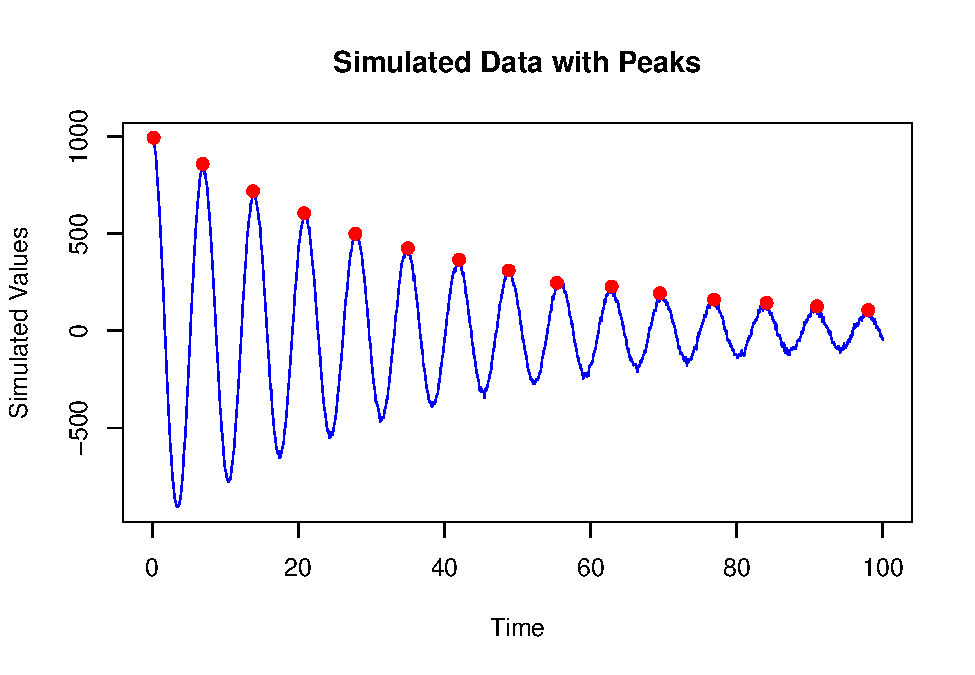
\includegraphics{CircadianProjectForMcManus_files/figure-latex/unnamed-chunk-9-1.pdf}
\#\#Finding initial parameters:A and gamma

\begin{Shaded}
\begin{Highlighting}[]
\CommentTok{\# transform into log}
\NormalTok{log\_y\_peaks }\OtherTok{\textless{}{-}} \FunctionTok{log}\NormalTok{(y\_peaks)}

\CommentTok{\# logy = {-}gamma*t + logA}
\NormalTok{fit\_linear }\OtherTok{\textless{}{-}} \FunctionTok{lm}\NormalTok{(log\_y\_peaks }\SpecialCharTok{\textasciitilde{}}\NormalTok{ t\_peaks) }

\FunctionTok{summary}\NormalTok{(fit\_linear)}
\end{Highlighting}
\end{Shaded}

\begin{verbatim}
## 
## Call:
## lm(formula = log_y_peaks ~ t_peaks)
## 
## Residuals:
##       Min        1Q    Median        3Q       Max 
## -0.096938 -0.017879 -0.002984  0.026874  0.049729 
## 
## Coefficients:
##              Estimate Std. Error t value Pr(>|t|)    
## (Intercept)  6.876027   0.019252  357.16   <2e-16 ***
## t_peaks     -0.022952   0.000335  -68.52   <2e-16 ***
## ---
## Signif. codes:  0 '***' 0.001 '**' 0.01 '*' 0.05 '.' 0.1 ' ' 1
## 
## Residual standard error: 0.03923 on 13 degrees of freedom
## Multiple R-squared:  0.9972, Adjusted R-squared:  0.997 
## F-statistic:  4694 on 1 and 13 DF,  p-value: < 2.2e-16
\end{verbatim}

\begin{Shaded}
\begin{Highlighting}[]
\CommentTok{\# get log(A)  and  gamma}
\NormalTok{log\_A }\OtherTok{\textless{}{-}} \FunctionTok{coef}\NormalTok{(fit\_linear)[}\DecValTok{1}\NormalTok{]}

\NormalTok{init\_gamma }\OtherTok{\textless{}{-}} \SpecialCharTok{{-}}\FunctionTok{coef}\NormalTok{(fit\_linear)[}\DecValTok{2}\NormalTok{] }\CommentTok{\#Extract gamma from the linear fit}

\FunctionTok{cat}\NormalTok{(}\StringTok{"log(A) ="}\NormalTok{, log\_A, }\StringTok{"}\SpecialCharTok{\textbackslash{}n}\StringTok{"}\NormalTok{)}
\end{Highlighting}
\end{Shaded}

\begin{verbatim}
## log(A) = 6.876027
\end{verbatim}

\begin{Shaded}
\begin{Highlighting}[]
\FunctionTok{cat}\NormalTok{(}\StringTok{"gamma ="}\NormalTok{, init\_gamma, }\StringTok{"}\SpecialCharTok{\textbackslash{}n}\StringTok{"}\NormalTok{)}
\end{Highlighting}
\end{Shaded}

\begin{verbatim}
## gamma = 0.02295209
\end{verbatim}

\begin{Shaded}
\begin{Highlighting}[]
\NormalTok{init\_A}\OtherTok{=}\FunctionTok{exp}\NormalTok{(log\_A)}
\FunctionTok{print}\NormalTok{(init\_A)}
\end{Highlighting}
\end{Shaded}

\begin{verbatim}
## (Intercept) 
##    968.7701
\end{verbatim}

\hypertarget{to-see-whether-the-initial-params-a-and-gamma-is-fitted-or-not}{%
\subsection{to see whether the initial params A and gamma is fitted or
not}\label{to-see-whether-the-initial-params-a-and-gamma-is-fitted-or-not}}

\begin{Shaded}
\begin{Highlighting}[]
\CommentTok{\#Plot the simulated data}
\FunctionTok{plot}\NormalTok{(t, y\_sim, }\AttributeTok{type =} \StringTok{"l"}\NormalTok{, }\AttributeTok{col =} \StringTok{"blue"}\NormalTok{, }\AttributeTok{main =} \StringTok{"Simulated Data with Fitted Exponential"}\NormalTok{, }\AttributeTok{xlab =} \StringTok{"Time"}\NormalTok{, }\AttributeTok{ylab =} \StringTok{"Simulated Values"}\NormalTok{)}

\CommentTok{\# Calculate the fitted exponential curve using estimated A and gamma from the linear model}
\NormalTok{init\_A }\OtherTok{\textless{}{-}} \FunctionTok{exp}\NormalTok{(log\_A)  }\CommentTok{\# Extract log\_A from the linear model}

\CommentTok{\# Add the fitted exponential curve}
\FunctionTok{curve}\NormalTok{(init\_A }\SpecialCharTok{*} \FunctionTok{exp}\NormalTok{(}\SpecialCharTok{{-}}\NormalTok{init\_gamma }\SpecialCharTok{*}\NormalTok{ x), }\AttributeTok{from =} \DecValTok{0}\NormalTok{, }\AttributeTok{to =} \FunctionTok{max}\NormalTok{(t), }\AttributeTok{col =} \StringTok{"green"}\NormalTok{, }\AttributeTok{add =} \ConstantTok{TRUE}\NormalTok{, }\AttributeTok{lwd =} \DecValTok{2}\NormalTok{)}
\CommentTok{\#  Add a legend }
\FunctionTok{legend}\NormalTok{(}\StringTok{"topright"}\NormalTok{, }\AttributeTok{legend =} \FunctionTok{c}\NormalTok{(}\StringTok{"Simulated Data"}\NormalTok{, }\StringTok{"Fitted Exponential"}\NormalTok{), }\AttributeTok{col =} \FunctionTok{c}\NormalTok{(}\StringTok{"blue"}\NormalTok{, }\StringTok{"green"}\NormalTok{), }\AttributeTok{lty =} \DecValTok{1}\NormalTok{)}
\end{Highlighting}
\end{Shaded}

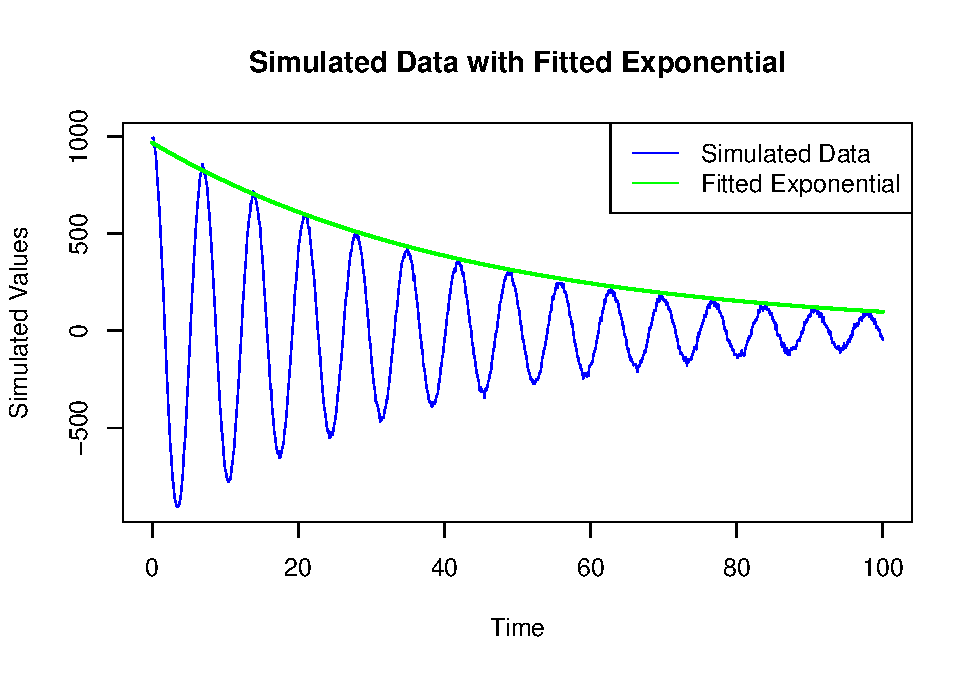
\includegraphics{CircadianProjectForMcManus_files/figure-latex/unnamed-chunk-11-1.pdf}

\#\#find initial value:omega

\begin{Shaded}
\begin{Highlighting}[]
\CommentTok{\# Extract the time points of the first two consecutive maxima from t\_peaks}
\NormalTok{t\_max1 }\OtherTok{\textless{}{-}}\NormalTok{ t\_peaks[}\DecValTok{1}\NormalTok{]  }\CommentTok{\# First maximum}
\NormalTok{t\_max2 }\OtherTok{\textless{}{-}}\NormalTok{ t\_peaks[}\DecValTok{2}\NormalTok{]  }\CommentTok{\# Second maximum}

\CommentTok{\# Calculate the time difference between two consecutive maxima}
\NormalTok{Delta }\OtherTok{\textless{}{-}}\NormalTok{ t\_max2 }\SpecialCharTok{{-}}\NormalTok{ t\_max1}

\CommentTok{\# Estimate omega (tau) using the formula 2*pi/Delta}
\NormalTok{init\_omega }\OtherTok{\textless{}{-}} \DecValTok{2} \SpecialCharTok{*}\NormalTok{ pi }\SpecialCharTok{/}\NormalTok{ Delta}

\CommentTok{\# Output the result}
\FunctionTok{cat}\NormalTok{(}\StringTok{"initial omega (tau) ="}\NormalTok{, init\_omega, }\StringTok{"}\SpecialCharTok{\textbackslash{}n}\StringTok{"}\NormalTok{)}
\end{Highlighting}
\end{Shaded}

\begin{verbatim}
## initial omega (tau) = 0.9377889
\end{verbatim}

\begin{Shaded}
\begin{Highlighting}[]
\FunctionTok{cat}\NormalTok{(}\StringTok{"Time difference between consecutive maxima (Delta) ="}\NormalTok{, Delta, }\StringTok{"}\SpecialCharTok{\textbackslash{}n}\StringTok{"}\NormalTok{)}
\end{Highlighting}
\end{Shaded}

\begin{verbatim}
## Time difference between consecutive maxima (Delta) = 6.7
\end{verbatim}

we assume period delta keeps same. now our initial parameters are{[}A =
968.7701,gamma = 0.02295209 ,omega = 0.9377889 , phi = 0, y\_shift =
0{]}

\#\#estimate parameter for simulating data for 1 time using initial
parameters, and use mle

\begin{Shaded}
\begin{Highlighting}[]
\CommentTok{\# }
\NormalTok{log\_likelihood\_dnorm }\OtherTok{\textless{}{-}} \ControlFlowTok{function}\NormalTok{(params, t, y\_obs) \{}
\NormalTok{  A }\OtherTok{\textless{}{-}}\NormalTok{ params[}\DecValTok{1}\NormalTok{]}
\NormalTok{  gamma }\OtherTok{\textless{}{-}}\NormalTok{ params[}\DecValTok{2}\NormalTok{]}
\NormalTok{  omega }\OtherTok{\textless{}{-}}\NormalTok{ params[}\DecValTok{3}\NormalTok{]}
\NormalTok{  phi }\OtherTok{\textless{}{-}}\NormalTok{ params[}\DecValTok{4}\NormalTok{]}
\NormalTok{  y\_shift }\OtherTok{\textless{}{-}}\NormalTok{ params[}\DecValTok{5}\NormalTok{]}
\NormalTok{  sigma }\OtherTok{\textless{}{-}}\NormalTok{ params[}\DecValTok{6}\NormalTok{] }
\NormalTok{  y\_pred }\OtherTok{\textless{}{-}} \FunctionTok{model\_function}\NormalTok{(t, A, gamma, omega, phi, y\_shift)}
\NormalTok{  logL }\OtherTok{\textless{}{-}} \FunctionTok{sum}\NormalTok{(}\FunctionTok{dnorm}\NormalTok{(y\_obs, }\AttributeTok{mean =}\NormalTok{ y\_pred, }\AttributeTok{sd =}\NormalTok{ sigma, }\AttributeTok{log =} \ConstantTok{TRUE}\NormalTok{))}
  
  \FunctionTok{return}\NormalTok{(}\SpecialCharTok{{-}}\NormalTok{logL) }
\NormalTok{\}}

\CommentTok{\#unkown params}
\NormalTok{initial\_params }\OtherTok{\textless{}{-}} \FunctionTok{c}\NormalTok{(}\AttributeTok{A =} \FloatTok{968.7701}\NormalTok{,}\AttributeTok{gamma =} \FloatTok{0.02295209}\NormalTok{ ,}\AttributeTok{omega =} \FloatTok{0.9377889}\NormalTok{ , }\AttributeTok{phi =} \DecValTok{0}\NormalTok{, }\AttributeTok{y\_shift =} \DecValTok{0}\NormalTok{,}\AttributeTok{sigma =}\DecValTok{10}\NormalTok{)}


\NormalTok{fit\_mle }\OtherTok{\textless{}{-}} \FunctionTok{optim}\NormalTok{(}\AttributeTok{par =}\NormalTok{ initial\_params, }
                 \AttributeTok{fn =}\NormalTok{ log\_likelihood\_dnorm, }
                 \AttributeTok{t =}\NormalTok{ t, }
                 \AttributeTok{y\_obs =}\NormalTok{ y\_sim, }
                 \AttributeTok{method =} \StringTok{"L{-}BFGS{-}B"}\NormalTok{, }
                 \AttributeTok{lower =} \FunctionTok{c}\NormalTok{(}\DecValTok{0}\NormalTok{, }\DecValTok{0}\NormalTok{, }\DecValTok{0}\NormalTok{, }\SpecialCharTok{{-}}\NormalTok{pi, }\SpecialCharTok{{-}}\ConstantTok{Inf}\NormalTok{, }\FloatTok{0.00001}\NormalTok{), }\CommentTok{\#avoid 0 sigma}
                 \AttributeTok{upper =} \FunctionTok{c}\NormalTok{(}\ConstantTok{Inf}\NormalTok{, }\ConstantTok{Inf}\NormalTok{, }\ConstantTok{Inf}\NormalTok{, pi, }\ConstantTok{Inf}\NormalTok{, }\ConstantTok{Inf}\NormalTok{))}


\NormalTok{estimated\_params }\OtherTok{\textless{}{-}}\NormalTok{ fit\_mle}\SpecialCharTok{$}\NormalTok{par}
\FunctionTok{print}\NormalTok{(}\FunctionTok{round}\NormalTok{(estimated\_params,}\DecValTok{3}\NormalTok{))}
\end{Highlighting}
\end{Shaded}

\begin{verbatim}
##       A   gamma   omega     phi y_shift   sigma 
## 968.770   0.024   0.900  -0.002   0.000  10.003
\end{verbatim}

Detrending the Data (Exponential Method)

\begin{Shaded}
\begin{Highlighting}[]
\CommentTok{\# \# Define detrending function using exponential method}
\CommentTok{\# detrend\_exponential \textless{}{-} function(time, data\_column) \{}
\CommentTok{\#   \# Fit an exponential model}
\CommentTok{\#   trend\_model\_exp \textless{}{-} lm(log(data\_column) \textasciitilde{} time)}
\CommentTok{\#   }
\CommentTok{\#   \# Detrend the data by subtracting the fitted exponential trend}
\CommentTok{\#   detrended\_data \textless{}{-} data\_column {-} exp(fitted(trend\_model\_exp))}
\CommentTok{\#   }
\CommentTok{\#   return(detrended\_data)}
\CommentTok{\# \}}
\CommentTok{\# }
\CommentTok{\# \# Apply detrending to each column}
\CommentTok{\# detrended\_X1 \textless{}{-} detrend\_exponential(df\_MC$Time, df\_MC$X1)}
\CommentTok{\# detrended\_X2 \textless{}{-} detrend\_exponential(df\_MC$Time, df\_MC$X2)}
\CommentTok{\# detrended\_X3 \textless{}{-} detrend\_exponential(df\_MC$Time, df\_MC$X3)}
\CommentTok{\# detrended\_X4 \textless{}{-} detrend\_exponential(df\_MC$Time, df\_MC$X4)}
\CommentTok{\# }
\CommentTok{\# \# Plot detrended data}
\CommentTok{\# plot(df\_MC$Time, detrended\_X1, type = "l", col = "blue", xlab = "Time", ylab = "Detrended Values", }
\CommentTok{\#      main = "Detrended X1, X2, X3, X4 (Exponential)")}
\CommentTok{\# lines(df\_MC$Time, detrended\_X2, type = "l", col = "green")}
\CommentTok{\# lines(df\_MC$Time, detrended\_X3, type = "l", col = "red")}
\CommentTok{\# lines(df\_MC$Time, detrended\_X4, type = "l", col = "purple")}
\CommentTok{\# }
\CommentTok{\# legend("topright", legend = c("X1", "X2", "X3", "X4"), col = c("blue", "green", "red", "purple"), lty = 1, cex = 0.8)}
\end{Highlighting}
\end{Shaded}

Spline Smooth

\begin{Shaded}
\begin{Highlighting}[]
\CommentTok{\# \# Spline smoothing for detrended data}
\CommentTok{\# spline\_detrend\_X1 \textless{}{-} predict(smooth.spline(df\_MC$Time, detrended\_X1))}
\CommentTok{\# spline\_detrend\_X2 \textless{}{-} predict(smooth.spline(df\_MC$Time, detrended\_X2))}
\CommentTok{\# spline\_detrend\_X3 \textless{}{-} predict(smooth.spline(df\_MC$Time, detrended\_X3))}
\CommentTok{\# spline\_detrend\_X4 \textless{}{-} predict(smooth.spline(df\_MC$Time, detrended\_X4))}
\CommentTok{\# }
\CommentTok{\# \# Plot the spline{-}smoothed data}
\CommentTok{\# plot(df\_MC$Time, spline\_detrend\_X1$y, type = "l", col = "red", lwd = 2, }
\CommentTok{\#      xlab = "Time", ylab = "Values", main = "Detrended Splines", }
\CommentTok{\#      ylim = range(c(spline\_detrend\_X1$y, spline\_detrend\_X2$y, spline\_detrend\_X3$y, spline\_detrend\_X4)))}
\CommentTok{\# lines(df\_MC$Time, spline\_detrend\_X2$y, col = "blue", lwd = 2)}
\CommentTok{\# lines(df\_MC$Time, spline\_detrend\_X3$y, col = "green", lwd = 2)}
\CommentTok{\# lines(df\_MC$Time, spline\_detrend\_X4$y, col = "purple", lwd = 2)}
\CommentTok{\# }
\CommentTok{\# legend("topright", legend = c("spline\_detrend\_X1", "spline\_detrend\_X2", "spline\_detrend\_X3", "spline\_detrend\_X4"), }
\CommentTok{\#        col = c("red", "blue", "green", "purple"), lwd = 2)}
\end{Highlighting}
\end{Shaded}

Nonlinear Least Squares Model Fitting with Weights \#\#time specific

\begin{Shaded}
\begin{Highlighting}[]
\CommentTok{\# Define the model function}
\NormalTok{model\_function }\OtherTok{\textless{}{-}} \ControlFlowTok{function}\NormalTok{(t, A, gamma, omega, phi, y\_shift) \{}
\NormalTok{  A }\SpecialCharTok{*} \FunctionTok{exp}\NormalTok{(}\SpecialCharTok{{-}}\NormalTok{gamma }\SpecialCharTok{*}\NormalTok{ t ) }\SpecialCharTok{*} \FunctionTok{cos}\NormalTok{(omega }\SpecialCharTok{*}\NormalTok{ t }\SpecialCharTok{+}\NormalTok{ phi) }\SpecialCharTok{+}\NormalTok{ y\_shift}
\NormalTok{\}}
\CommentTok{\# Function to calculate variance at each time point}
\NormalTok{calculate\_variance }\OtherTok{\textless{}{-}} \ControlFlowTok{function}\NormalTok{(replicates) \{}
\NormalTok{  n }\OtherTok{\textless{}{-}} \FunctionTok{nrow}\NormalTok{(replicates)}
\NormalTok{  mean\_vals }\OtherTok{\textless{}{-}} \FunctionTok{rowMeans}\NormalTok{(replicates)  }\CommentTok{\# Mean for each time point}
\NormalTok{  variance }\OtherTok{\textless{}{-}} \FunctionTok{rowSums}\NormalTok{((replicates }\SpecialCharTok{{-}}\NormalTok{ mean\_vals)}\SpecialCharTok{\^{}}\DecValTok{2}\NormalTok{) }\SpecialCharTok{/}\NormalTok{ (n }\SpecialCharTok{{-}} \DecValTok{1}\NormalTok{)  }\CommentTok{\# Variance formula}
  \FunctionTok{return}\NormalTok{(variance)}
\NormalTok{\}}
\CommentTok{\# Weighted nonlinear least squares estimation}
\NormalTok{weighted\_nls }\OtherTok{\textless{}{-}} \ControlFlowTok{function}\NormalTok{(t, replicates, initial\_params) \{}
\NormalTok{  variances }\OtherTok{\textless{}{-}} \FunctionTok{calculate\_variance}\NormalTok{(replicates)  }\CommentTok{\# Variance at each time point}

  \CommentTok{\# Fit the model using nlsLM}
\NormalTok{  fit }\OtherTok{\textless{}{-}} \FunctionTok{nlsLM}\NormalTok{(y }\SpecialCharTok{\textasciitilde{}} \FunctionTok{model\_function}\NormalTok{(t, A, gamma, omega, phi, y\_shift),}
               \AttributeTok{start =}\NormalTok{ initial\_params,}
               \AttributeTok{data =} \FunctionTok{list}\NormalTok{(}\AttributeTok{t =}\NormalTok{ t, }\AttributeTok{y =} \FunctionTok{rowMeans}\NormalTok{(replicates)),}
               \AttributeTok{weights =} \DecValTok{1} \SpecialCharTok{/}\NormalTok{ variances)  }\CommentTok{\# Weight by the inverse of variances}
  \FunctionTok{return}\NormalTok{(fit)}
\NormalTok{\}}
\CommentTok{\# Use data from replicates for fitting}
\NormalTok{replicates }\OtherTok{\textless{}{-}}\NormalTok{ df\_MC[, }\FunctionTok{c}\NormalTok{(}\StringTok{"X1"}\NormalTok{, }\StringTok{"X2"}\NormalTok{, }\StringTok{"X3"}\NormalTok{, }\StringTok{"X4"}\NormalTok{)]}
\CommentTok{\# Calculate variance}
\NormalTok{variances }\OtherTok{\textless{}{-}} \FunctionTok{calculate\_variance}\NormalTok{(replicates)}
\FunctionTok{hist}\NormalTok{(variances, }\AttributeTok{main =} \StringTok{"Histogram of Variances"}\NormalTok{,}
     \AttributeTok{xlab =} \StringTok{"Variance"}\NormalTok{,}
     \AttributeTok{ylab =} \StringTok{"Frequency"}\NormalTok{,}
     \AttributeTok{col =} \StringTok{"lightblue"}\NormalTok{,}
     \AttributeTok{border =} \StringTok{"black"}\NormalTok{)}
\end{Highlighting}
\end{Shaded}

\includegraphics{CircadianProjectForMcManus_files/figure-latex/unnamed-chunk-16-1.pdf}

\begin{Shaded}
\begin{Highlighting}[]
\CommentTok{\# Initial parameter estimates}
\NormalTok{param0}\OtherTok{=}\FunctionTok{c}\NormalTok{(}\AttributeTok{A=} \DecValTok{1000}\NormalTok{, }\AttributeTok{gamma =} \FloatTok{0.025}\NormalTok{,}\AttributeTok{omega =} \FloatTok{0.9}\NormalTok{,}\AttributeTok{phi=} \DecValTok{0}\NormalTok{,}\AttributeTok{y\_shift =} \DecValTok{0}\NormalTok{)}
\CommentTok{\# Perform weighted nonlinear least squares fitting}
\NormalTok{fit }\OtherTok{\textless{}{-}} \FunctionTok{weighted\_nls}\NormalTok{(df\_MC}\SpecialCharTok{$}\NormalTok{Time, replicates, param0)}
\CommentTok{\# Print estimated parameters}
\NormalTok{estimated\_params }\OtherTok{\textless{}{-}} \FunctionTok{coef}\NormalTok{(fit)}
\FunctionTok{print}\NormalTok{(estimated\_params)}
\end{Highlighting}
\end{Shaded}

\begin{verbatim}
##             A         gamma         omega           phi       y_shift 
##  6.475202e+01  1.252247e-04  1.037711e+00 -5.216541e-01  5.024669e+02
\end{verbatim}

\end{document}
